\documentclass[12pt]{article}
\usepackage[table]{xcolor}
\usepackage[shortlabels]{enumitem}
\usepackage{tabularx,xltabular}
\usepackage{graphicx}
\usepackage{hyperref}
\usepackage{verbatim}
\usepackage{geometry}
\usepackage{ulem}
\usepackage[official]{eurosym}
\usepackage{tikz}
\usetikzlibrary{arrows,backgrounds,calc,decorations.markings,patterns,3d,positioning,fit,angles, quotes}
\usepackage{pgfplots}
\pgfplotsset{compat = newest}
\usetikzlibrary{fit}
\newcommand\addvmargin[1]{
\usetikzlibrary{arrows}
\node[fit=(current bounding box),inner ysep=#1,inner xsep=0]{};}
\usepackage{cancel}
\usepackage{fontspec}
\usepackage{array}  
\geometry{a4paper, top=2cm, left=2cm, right=2cm, bottom=2cm, headsep=1cm}
\usepackage{tabu}
\usepackage{pst-node}
\usepackage{colortbl}
\usepackage{array}
\usepackage{german}
\setlength\parindent{0pt}
\newcolumntype{?}{!{\vrule width 1pt}}
\usepackage{makecell}
\renewcommand{\arraystretch}{2.5}
\usepackage{pbox}
\usepackage{amssymb}
\usepackage{amsmath}
\usepackage{booktabs}
\newcolumntype{L}[1]{>{\raggedright\let\newline\\\arraybackslash\hspace{0pt}}m{#1}}
\newcolumntype{C}[1]{>{\centering\let\newline\\\arraybackslash\hspace{0pt}}m{#1}}
\newcolumntype{R}[1]{>{\raggedleft\let\newline\\\arraybackslash\hspace{0pt}}m{#1}}
\begin{document}
\pgfmathsetmacro{\pkteAfgEins}{3}
\pgfmathsetmacro{\pkteAfgZwei}{4}
\pgfmathsetmacro{\pkteAfgDrei}{4}
\pgfmathsetmacro{\pkteAfgVier}{2}
\pgfmathsetmacro{\pkteAfgFuenf}{8}
\pgfmathsetmacro{\pkteAfgSechs}{0}
\pgfmathsetmacro{\pkteAfgSieben}{0}
\pgfmathsetmacro{\sauberkeitsPkte}{2}
\def\datum{12.12.2023}
\def\kurs{~}
\def\titel{Flächen und Umfänge}
\def\jahr{2022/2023}
\def\fach{Mathematik}
\def\name{~}
\def\material{Füller / Kugelschreiber / Fineliner, Bleistift, Taschenrechner}
\pgfmathsetmacro{\gesPkte}{\pkteAfgEins+\pkteAfgZwei+\pkteAfgDrei+\pkteAfgVier+\pkteAfgFuenf+\pkteAfgSechs+\pkteAfgSieben+\sauberkeitsPkte}
%Mit den folgenden Zeilen werden die Nummern nicht angezeigt, bei denen die Aufgaben 0 Punkte haben.
\newcommand{\Eins}{~}
\newcommand{\pEins}{~}
\ifnum\pkteAfgEins>0  \renewcommand{\Eins}{1} \fi
\ifnum\pkteAfgEins>0  \renewcommand{\pEins}{\pkteAfgEins} \fi
\newcommand{\Zwei}{~}
\newcommand{\pZwei}{~}
\ifnum\pkteAfgZwei>0  \renewcommand{\Zwei}{2} \fi
\ifnum\pkteAfgZwei>0  \renewcommand{\pZwei}{\pkteAfgZwei} \fi
\newcommand{\Drei}{~}
\newcommand{\pDrei}{~}
\ifnum\pkteAfgDrei>0  \renewcommand{\Drei}{3} \fi
\ifnum\pkteAfgDrei>0  \renewcommand{\pDrei}{\pkteAfgDrei} \fi
\newcommand{\Vier}{~}
\newcommand{\pVier}{~}
\ifnum\pkteAfgVier>0  \renewcommand{\Vier}{4} \fi
\ifnum\pkteAfgVier>0  \renewcommand{\pVier}{\pkteAfgVier} \fi
\newcommand{\Fuenf}{~}
\newcommand{\pFuenf}{~}
\ifnum\pkteAfgFuenf>0  \renewcommand{\Fuenf}{5} \fi
\ifnum\pkteAfgFuenf>0  \renewcommand{\pFuenf}{\pkteAfgFuenf} \fi
\newcommand{\Sechs}{~}
\newcommand{\pSechs}{~}
\ifnum\pkteAfgSechs>0  \renewcommand{\Sechs}{6} \fi
\ifnum\pkteAfgSechs>0  \renewcommand{\pSechs}{\pkteAfgSechs} \fi
\newcommand{\Sieben}{~}
\newcommand{\pSieben}{~}
\ifnum\pkteAfgSieben>0  \renewcommand{\Sieben}{7} \fi
\ifnum\pkteAfgSieben>0  \renewcommand{\pSieben}{\pkteAfgSieben} \fi
\newcommand{\sauber}{~}
\newcommand{\pSauber}{~}
\ifnum\sauberkeitsPkte>0  \renewcommand{\sauber}{SK} \fi
\ifnum\sauberkeitsPkte>0  \renewcommand{\pSauber}{\sauberkeitsPkte} \fi
\pagenumbering{gobble}
\begin{tabularx}{\textwidth}{ R{2.0cm} X R{2.0cm}  }
&
{\centering{\Large\bf
\fach\\
\titel}\\ 
Schuljahr \jahr\par
} &
\end{tabularx} \\
\begin{tabularx}{\textwidth}{R{2.0cm} X R{2.0cm} X }
Name: & \name& Kurs:  & \kurs\\\cline{2-2}\cline{4-4}
& & Datum:& \datum \\\cline{2-2}\cline{4-4}
\end{tabularx} \\
\phantom{M}\\
{\bf\underline{Benötigtes Material}}\\
\vspace{-0.5cm}
\begin{itemize}
\itemsep0em 
\foreach \x in \material
{\item \x }
\end{itemize}

{\bf\underline{Ablauf:}}\\
Nach dem Verteilen der Arbeit schreibst du auf jedem Zettel deinen Namen. Lege danach dein Stift wieder weg. Wenn alle die Arbeit haben, fangen wir an. Du hast 45 min Zeit zur Bearbeitung der Aufgaben.
\\
{\bf\underline{Allgemeines:}}\\
\vspace{-0.5cm}
\begin{enumerate}
\itemsep0em 
\item Während der Arbeit darf nicht miteinander gesprochen werden. Willst Du was sagen, melde dich.
\item Wenn Dir eine Aufgabenstellung unklar ist, melde Dich.
\item Wer schummelt hat verloren!
\end{enumerate}

\begin{tabularx}{\textwidth}{|X|C{1cm}|C{1cm}|C{1cm}|C{1cm}|C{1cm}|C{1cm}|C{1cm}|C{1cm}|C{1cm}|}
\hline
Aufgabe & \Eins&\Zwei&\Drei&\Vier&\Fuenf&\Sechs&\Sieben& \sauber & $\sum$ \\\hline
Mögliche Punkte &\pEins&\pZwei&\pDrei&\pVier&\pFuenf&\pSechs&\pSieben&  \pSauber&\pgfmathprintnumber{\gesPkte} \\\hline
Erreichte Punkte& & & & & & & &  & \\\hline
\end{tabularx}\\
\phantom{M} \\
\begin{tabularx}{\textwidth}{|c| }
\hline 
{\bf Erreichte Note}\\\hline
\parbox[c][3cm]{16.55cm}{\phantom{M}} \\\hline
\end{tabularx} 
{\centering{\large\bf
Gleich geht’s los! Viel Erfolg!
\par
}}
\newpage
\pagenumbering{arabic}
\pgfmathsetmacro{\punkte}{\pkteAfgEins}
\newpage
\section{Gleichungen}
\subsection{Gl. lösen Mal und Minus}
Füge hier bitte einen Beschreibungstext ein. Behalte die beiden Backslash \textbackslash\textbackslash. Die bedeuten eine neue Zeile. Soll die Aufgabe nicht auf einer neuen Seite beginnen, entferne den Befehl \textbackslash newpage am Anfang der tex-Datei.\\
\begin{xltabular}{\textwidth}{|C{0.75cm}|X|}
\arrayrulecolor{black}\hline
a)&$10\cdot a-11=19$
\\\hline
\end{xltabular}
\vspace{0.5cm}
\subsection{Gl. nur mit Mal/Geteilt lösen}
Füge hier bitte einen Beschreibungstext ein. Behalte die beiden Backslash \textbackslash\textbackslash. Die bedeuten eine neue Zeile. Soll die Aufgabe nicht auf einer neuen Seite beginnen, entferne den Befehl \textbackslash newpage am Anfang der tex-Datei.\\
\begin{xltabular}{\textwidth}{|C{0.75cm}|X|}
\arrayrulecolor{black}\hline
a)&$y:8=7$
\\\hline
\end{xltabular}
\vspace{0.5cm}
\subsection{Gleichung nur +/- lösen}
Füge hier bitte einen Beschreibungstext ein. Behalte die beiden Backslash \textbackslash\textbackslash. Die bedeuten eine neue Zeile. Soll die Aufgabe nicht auf einer neuen Seite beginnen, entferne den Befehl \textbackslash newpage am Anfang der tex-Datei.\\
\begin{xltabular}{\textwidth}{|C{0.75cm}|X|}
\arrayrulecolor{black}\hline
a)&$a-30 = 43$
\\\hline
\end{xltabular}
\vspace{0.5cm}
\begin{flushright}
\underline{\hspace{2cm}/ \punkte~Punkte}
\end{flushright}
\pgfmathsetmacro{\punkte}{\pkteAfgZwei}
\newpage
\section{Flächen und Umfänge}
\subsection{Dreieck Fl. Mit Beschr.}
Füge hier bitte einen Beschreibungstext ein. Behalte die beiden Backslash \textbackslash\textbackslash. Die bedeuten eine neue Zeile. Soll die Aufgabe nicht auf einer neuen Seite beginnen, entferne den Befehl \textbackslash newpage am Anfang der tex-Datei.\\
\begin{xltabular}{\textwidth}{|C{0.75cm}|X|}
\arrayrulecolor{black}\hline
a)&\pbox{5cm}{
\tikzstyle{background grid}=[draw, black!15,step=.5cm]
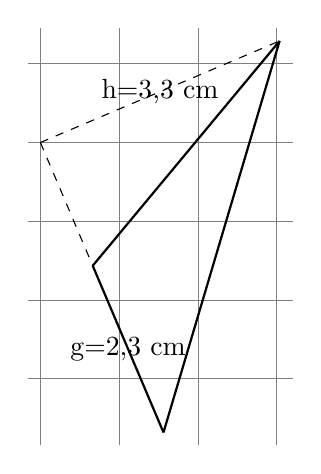
\begin{tikzpicture}[show background grid]
\draw[thick,black] (293:1.7000000000000002) -- node{g=2,3 cm} (293:4.0);
\draw[thick,black] (293:1.7000000000000002)  -- (383:3.3);
\draw[thick,black] (293:4.0)  -- (383:3.3);
\draw[dashed,black] (0,0)  -- node{h=3,3 cm} (383:3.3);
\draw[dashed,black] (0,0)  -- (293:1.7000000000000002);
\end{tikzpicture}
}
\\\hline
\end{xltabular}
\vspace{0.5cm}
\subsection{Trapez mit Beschr.}
Füge hier bitte einen Beschreibungstext ein. Behalte die beiden Backslash \textbackslash\textbackslash. Die bedeuten eine neue Zeile. Soll die Aufgabe nicht auf einer neuen Seite beginnen, entferne den Befehl \textbackslash newpage am Anfang der tex-Datei.\\
\begin{xltabular}{\textwidth}{|C{0.75cm}|X|}
\arrayrulecolor{black}\hline
a)&\pbox{5cm}{
\tikzstyle{background grid}=[draw, black!15,step=.5cm]
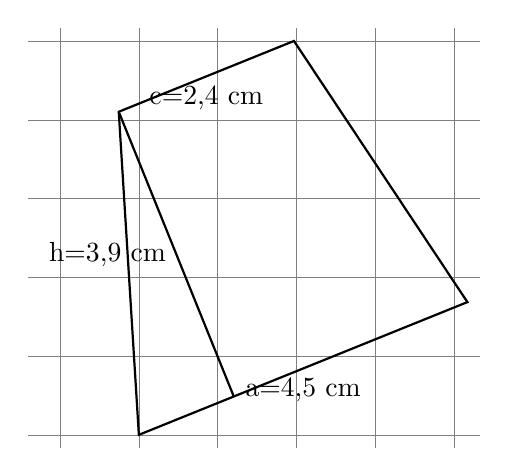
\begin{tikzpicture}[show background grid]
\draw[thick,black,rotate=22] (0,0) -- node[below]{a=4,5 cm} ++(4.5,0) -- ++(-0.8,3.9) --node[below]{c=2,4 cm} ++(-2.4,0) --cycle;
\draw[thick,black,rotate=22] (1.3,0) --node[left]{h=3,9 cm}  ++(0,3.9);
\end{tikzpicture}
}
\\\hline
\end{xltabular}
\vspace{0.5cm}
\subsection{Parallelogramm Fl. Mit Beschr.}
Füge hier bitte einen Beschreibungstext ein. Behalte die beiden Backslash \textbackslash\textbackslash. Die bedeuten eine neue Zeile. Soll die Aufgabe nicht auf einer neuen Seite beginnen, entferne den Befehl \textbackslash newpage am Anfang der tex-Datei.\\
\begin{xltabular}{\textwidth}{|C{0.75cm}|X|}
\arrayrulecolor{black}\hline
a)&\pbox{5cm}{
\tikzstyle{background grid}=[draw, black!15,step=.5cm]
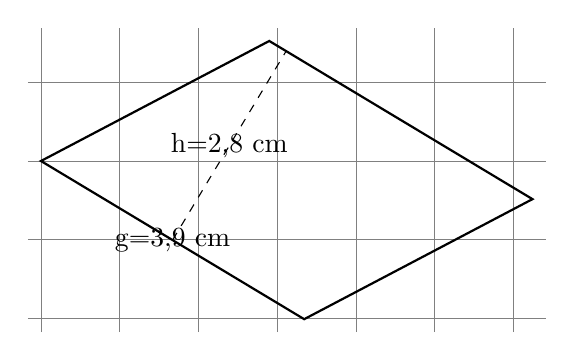
\begin{tikzpicture}[show background grid]
\draw[thick,black,rotate=329] (0,0) -- node{g=3,9 cm} ++(3.9,0) -- ++(1.7,2.8) -- ++(-3.9,0) --cycle;
\draw[dashed,black,rotate=329] (1.95,0)  -- node{h=2,8 cm} ++(0,2.8);
\end{tikzpicture}
}
\\\hline
\end{xltabular}
\vspace{0.5cm}
\subsection{Rechteck Fl. und Umf. bestimmen}
Füge hier bitte einen Beschreibungstext ein. Behalte die beiden Backslash \textbackslash\textbackslash. Die bedeuten eine neue Zeile. Soll die Aufgabe nicht auf einer neuen Seite beginnen, entferne den Befehl \textbackslash newpage am Anfang der tex-Datei.\\
\begin{xltabular}{\textwidth}{|C{0.75cm}|X|}
\arrayrulecolor{black}\hline
a)&\tikzstyle{background grid}=[draw, black!15,step=.5cm]
\noindent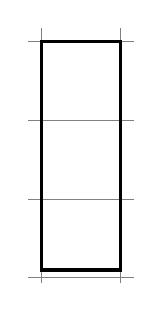
\begin{tikzpicture}[show background grid]
\draw[black, very thick] (0cm,0.1cm) rectangle (1cm,3cm);
\end{tikzpicture}
\\\hline
\end{xltabular}
\vspace{0.5cm}
\begin{flushright}
\underline{\hspace{2cm}/ \punkte~Punkte}
\end{flushright}
\pgfmathsetmacro{\punkte}{\pkteAfgDrei}
\newpage
\section{Terme}
\subsection{Werte Einsetzen}
Füge hier bitte einen Beschreibungstext ein. Behalte die beiden Backslash \textbackslash\textbackslash. Die bedeuten eine neue Zeile. Soll die Aufgabe nicht auf einer neuen Seite beginnen, entferne den Befehl \textbackslash newpage am Anfang der tex-Datei.\\
\begin{xltabular}{\textwidth}{|C{0.75cm}|X|}
\arrayrulecolor{black}\hline
a)& $a=9~ \rightarrow ~ 3 \cdot a + 4 \cdot a=?$
\\\hline
b)& $a=-1~ \rightarrow ~ 2 \cdot a + 4 \cdot a=?$
\\\hline
\end{xltabular}
\vspace{0.5cm}
\subsection{Terme umformen HS}
Füge hier bitte einen Beschreibungstext ein. Behalte die beiden Backslash \textbackslash\textbackslash. Die bedeuten eine neue Zeile. Soll die Aufgabe nicht auf einer neuen Seite beginnen, entferne den Befehl \textbackslash newpage am Anfang der tex-Datei.\\
\begin{xltabular}{\textwidth}{|C{0.75cm}|X|}
\arrayrulecolor{black}\hline
a)&$2 + 3 - 1=?$
\\\hline
b)&$4 + 2 + x - 4x=?$
\\\hline
\end{xltabular}
\vspace{0.5cm}
\begin{flushright}
\underline{\hspace{2cm}/ \punkte~Punkte}
\end{flushright}
\pgfmathsetmacro{\punkte}{\pkteAfgVier}
\newpage
\section{Formeln}
Füge hier bitte einen Beschreibungstext ein. Behalte die beiden Backslash \textbackslash\textbackslash. Die bedeuten eine neue Zeile. Soll die Aufgabe nicht auf einer neuen Seite beginnen, entferne den Befehl \textbackslash newpage am Anfang der tex-Datei.\\
\begin{xltabular}{\textwidth}{|C{0.75cm}|X|}
\arrayrulecolor{black}\hline
a)&Parallelogramm:  $A=37,62~cm^2$, $a=3,7~cm$ und $h_b=3,8~cm$.
\\\hline
b)&Dreieck:  $A=18,98~cm^2$, $a=7,8~cm$, $c=9,1~cm$  und $h_b=5,2~cm$.
\\\hline
\end{xltabular}
\vspace{0.5cm}
\begin{flushright}
\underline{\hspace{2cm}/ \punkte~Punkte}
\end{flushright}
\pgfmathsetmacro{\punkte}{\pkteAfgFuenf}
\newpage
\section{Textaufgaben}
\begin{enumerate}[a)]
\item Bearbeite diese Liste nach bedarf.
\item Führe dazu folgende Schritte durch.
\begin{enumerate}[1.]
\item Das item ist ein Listeneintrag
\item Ändere items zu eigenen Aufgaben
\item Füge neue items hinzu.
\item Oder entferne die, die zu viel sind.
\end{enumerate}
\item Denke auch an die korrekte Punktevergabe.
\item Brauchst du keine Textaufgabe, lösche den Inhalt dieser Datei und setze die Punkte auf 0
\item Solltest du vor den Textaufgaben keine neue Seite wünschen, entferne den Befehl \textbackslash newpage.
\end{enumerate}
\begin{flushright}
\underline{\hspace{2cm}/ \punkte~Punkte}
\end{flushright}
\end{document}